\documentclass{article}
\usepackage{amsmath}
\usepackage{tikz}
\usetikzlibrary{math}

\begin{document}
\section{Test eval of pgfmathparse}
\subsection{Input precision}

\pgfmathparse{0}\pgfmathresult\\
\pgfmathparse{0.}\pgfmathresult\\
\pgfmathparse{0.0}\pgfmathresult\\
\pgfmathparse{0.00}\pgfmathresult\\
\pgfmathparse{0.000}\pgfmathresult\\
\pgfmathparse{0.0000}\pgfmathresult\\
\pgfmathparse{0.00000}\pgfmathresult\\
\pgfmathparse{0.000000}\pgfmathresult\\
\pgfmathparse{0.1}\pgfmathresult\\
\pgfmathparse{0.01}\pgfmathresult\\
\pgfmathparse{0.001}\pgfmathresult\\
\pgfmathparse{0.0001}\pgfmathresult\\
\pgfmathparse{0.00001}\pgfmathresult\\
\pgfmathparse{0.000001}\pgfmathresult\\
\pgfmathparse{0.0000001}\pgfmathresult\\
\pgfmathparse{1234567890123456789012345678901234567890123456789012345678901234567890123456789012345678901234567890}
\pgfmathresult\\
\pgfmathparse{1.2.3.4.5}\pgfmathresult\\
\pgfmathparse{1.1234567890123456789012345678901234567890123456789012345678901234567890123456789012345678901234567890}\pgfmathresult\\

\subsection{simple infix arithmetic}

\pgfmathparse{1-1}\pgfmathresult\\
\pgfmathparse{1-1.}\pgfmathresult\\
\pgfmathparse{1-1.0}\pgfmathresult\\
\pgfmathparse{1-1.00}\pgfmathresult\\
\pgfmathparse{1-1.000}\pgfmathresult\\
\pgfmathparse{1-1.0000}\pgfmathresult\\
\pgfmathparse{1-1.00000}\pgfmathresult\\
\pgfmathparse{1-1.000000}\pgfmathresult\\
\pgfmathparse{1.00001}\pgfmathresult\\
% TODO:
1.00002 = \pgfmathparse{1.00001-0}\pgfmathresult\\
1.00002 = \pgfmathparse{1.00001-0.0000076}\pgfmathresult\\
\pgfmathparse{1.00001-0.0000077}\pgfmathresult\\
\pgfmathparse{16383-0}\pgfmathresult\\ % largest allowed set

\subsection{unary signs}
\pgfmathparse{+0}\pgfmathresult\\
\pgfmathparse{-0}\pgfmathresult\\
\pgfmathparse{-0.000}\pgfmathresult\\
\pgfmathparse{+10}\pgfmathresult\\
\pgfmathparse{-10}\pgfmathresult\\
\pgfmathparse{+10.0}\pgfmathresult\\
\pgfmathparse{-10.0}\pgfmathresult\\
\pgfmathparse{+0.1}\pgfmathresult\\
\pgfmathparse{-0.1}\pgfmathresult\\
\pgfmathparse{-16383}
\pgfmathresult\\

\subsection{int}

\pgfmathparse{int(1-1.000000)}\pgfmathresult\\
\pgfmathparse{int(0)}\pgfmathresult\\
\pgfmathparse{int(0.)}\pgfmathresult\\
\pgfmathparse{int(0.0)}\pgfmathresult\\
\pgfmathparse{int(0.00)}\pgfmathresult\\
\pgfmathparse{int(0.000)}\pgfmathresult\\
\pgfmathparse{int(0.0000)}\pgfmathresult\\
\pgfmathparse{int(0.00000)}\pgfmathresult\\
\pgfmathparse{int(0.000000)}\pgfmathresult\\

\subsection{Unit arithmetic}

\pgfmathparse{3.pt}\pgfmathresult\\
\pgfmathparse{3.5pt}\pgfmathresult\\
\pgfmathparse{3.05pt}\pgfmathresult\\
\pgfmathparse{3.005pt}\pgfmathresult\\
\pgfmathparse{3.0005pt}\pgfmathresult\\
\pgfmathparse{3.00005pt}\pgfmathresult\\
\pgfmathparse{3.000005pt}\pgfmathresult\\
\pgfmathparse{3.0000005pt}\pgfmathresult\\
\pgfmathparse{2pt+3.5pt}\pgfmathresult\\
\pgfmathparse{2pt+3pt}\pgfmathresult\\
\pgfmathparse{2pt+3.0000005pt}\pgfmathresult\\

\subsection{Precision multiplication}

\pgfmathparse{10*2}\pgfmathresult\\
\pgfmathparse{10.0*2}\pgfmathresult\\
\pgfmathparse{10*2.0}\pgfmathresult\\

% TODO
20.20001 = \pgfmathparse{10.10*2.0}\pgfmathresult\\
20.01999 = \pgfmathparse{10.01*2.0}\pgfmathresult\\
20.00201 = \pgfmathparse{10.001*2.0}\pgfmathresult\\
20.00021 = \pgfmathparse{10.0001*2.0}\pgfmathresult\\
20.00003 = \pgfmathparse{10.00001*2.0}\pgfmathresult\\
\pgfmathparse{10.000001*2.0}\pgfmathresult\\
\pgfmathparse{10.0000001*2.0}\pgfmathresult\\
\pgfmathparse{10.00000001*2.0}\pgfmathresult\\

\subsection{Factorials}
\pgfmathparse{0!}\pgfmathresult\\
\pgfmathparse{1!}\pgfmathresult\\
\pgfmathparse{2!}\pgfmathresult\\
\pgfmathparse{3!}\pgfmathresult\\
\pgfmathparse{4!}\pgfmathresult\\
\pgfmathparse{5!}\pgfmathresult\\
\pgfmathparse{6!}\pgfmathresult\\
\pgfmathparse{7!}\pgfmathresult

\subsection{Function bare args}

cos left: \pgfmathparse{cos(180/5)}\pgfmathresult\\
cos right:\pgfmathparse{(cos 180)/5}\pgfmathresult\\
cos precedence: \pgfmathparse{cos 180/5}\pgfmathresult\\
% TODO
sin cos right: -0.01746 = \pgfmathparse{sin(cos 180)}\pgfmathresult\\
sin cos precedence: -0.01746 = \pgfmathparse{sin cos 180}\pgfmathresult\\

\clearpage
\subsection{Figure test}

\begin{figure}[h]
\centering
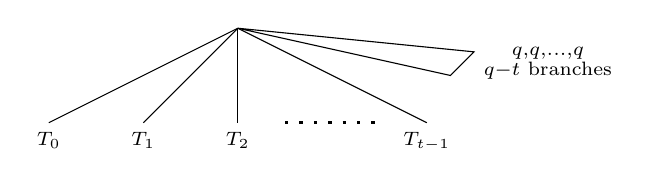
\begin{tikzpicture}[scale=1.2]
\draw(0,0)--(2.5,-0.25)--(2.25,-0.5)--(0,0);
\foreach[count=\j]\i in{-2,-1,0,2}{\draw(0,0)--(\i,-1);}\draw[very thick,loosely dotted](0.5,-1)--(1.5,-1);
\foreach[count=\j]\i in{-2,-1,0}{\tikzmath{\x=int(\j-1));}\node[below]at(\i,-1){$\substack{T_\x}$};}\node[below]at(2,-1){$\substack{T_{t-1}}$};
\node[right]at(2.5,-0.375){$\substack{q,q,\dotsc,q\\q-t\text{ branches}}$};
\end{tikzpicture}
\caption{The root of a tree diagram for $\mathcal{C}$}
\label{fig:rootq-node}
\end{figure}

\end{document}